\documentclass{article}
\usepackage[margin=1in]{geometry}

\usepackage{graphicx} % Required for inserting images
\usepackage{url}

\usepackage{listings}
\usepackage{xcolor}

\usepackage{tikz}
\usetikzlibrary{arrows.meta,shapes,positioning,calc}
\usepackage{subcaption}
\usepackage{alltt}
\usepackage{float}

\usepackage{amsmath}
\usepackage{amssymb}
\usepackage{listings}
\usepackage{booktabs}
\usepackage{hyperref}
\usepackage{cleveref}
\usepackage{booktabs}

\usepackage{hyperref}

\renewcommand{\lstlistingname}{Algorithm}



\lstset{
  language=Java,
  basicstyle=\ttfamily\small,
  frame=single,
  columns=fullflexible,
  keywordstyle=\bfseries,
  commentstyle=\itshape\color{gray},
  numbers=left,
  numberstyle=\tiny\color{gray},
  stepnumber=1,
  numbersep=8pt
}
 
\title{Implementing Side-Effect Analysis on a Modern Platform}
\author{Yuki Yang, Vivek Sarkar, Tijana Minic}
\date{March 2026}

\begin{document}

\maketitle


% a short (1-3 pages) project proposal that includes its thesis and technical approach.

\section{Motivation}
% Be sure to motivate your project. Your paper should start by stating the problem. It also should give a use case — essentially, a story about how the approach is used or what to learn from the proposed evaluation. For example, a software developer wants to perform a particular, realistic task, but cannot. Be specific about the problem and about why current techniques do not address it. Your approach solves that problem. An architectural diagram of how the pieces of your system fit together may be a useful summary.

% HAVE TO PARAPHRASE: In program understanding and documentation, the knowledge that a method is pure, or has no externally visible side effects, is especially useful because it guarantees that invocations of the method do not inadvertently interfere with other computations.

A function or method is side-effect-free if it does not modify any pre-existing program state; otherwise, it is \emph{side-effecting}. 
% In the absence of side-effect information, static analyses must conservatively assume that calls to external or library methods may modify arbitrary program state. This conservative assumption can destroy flow-sensitive information and significantly reduce analysis precision by discarding previously established invariants and prevents precise reasoning about program behavior, optimizations, or correctness.\newline
Side-effect freedom matters because: 
\begin{itemize}
\item Calling a side-effect-free function guarantees that no invariant in the caller can be modified \cite{salcianu2004combined}, simplifying reasoning about the code. Flow-sensitive refinements (e.g., “x is non-null here”, “receiver is unmodified”, “this alias set is stable”) can be preserved across calls that are known to be side-effect-free.
\item Side-effect-free methods are safe to reorder or duplicate, which is important, for example, in using commutativity to simplify the model in model checking.
\end{itemize}

Existing implementations \cite{helm2018unified, MadhavanPurity2011, salcianu2004combined} have either not been maintained or are not directly usable in verification frameworks.
%their output is \textcolor{red}{typically} not emitted in a format that can be directly consumed by verification tools. 

Our project's focus is solely on side-effect analysis. We aim to soundly compute side-effect information by inferring and validating side-effect summaries. Our contribution is not merely the implementation of a tool, but an empirical demonstration that static side-effect inference can (1) scale to widely used code and (2) improve the precision of downstream analyses that consume the side-effect information. \newline
% Clearly state the scientific question or contribution. For example, how is your project an (incremental) advance over previous work? Ideally, your results will be transferable to other domains: they will change the way that others think or act in the future, or provide guidance to programmers or to tool developers or both. Oftentimes, much of your project is not novel. That's OK — engineering is necessary in order to do experiments or to build on previous work — so long as you can point out the part that is novel. A new way of combining previously-known techniques is sufficiently novel.

\textbf{Contributions:}
\begin{itemize}
\item We implement Salcianu and Rinard's \cite{salcianu2004combined} heap side-effect analysis, providing the only extant runnable implementation to the best of our knowledge. This makes the analysis reproducible and enables its evaluation and use in modern Java analysis tooling.

\item We provide an empirical evaluation of the analysis on portions of the Java standard library, demonstrating its scalability and precision on real-world code and providing evidence that the analysis remains practical for modern Java codebases. \textcolor{red}{For Mike: Not sure what you meant by feedback on this bullet to compare with previous work to support or refute their claims. This is the only runnable implementation -- how are we supposed to compare?}

\item We demonstrate the practical utility of the inferred side-effect model by integrating it with downstream analysis tools (Checker Framework, Randoop, and Daikon), showing that the inferred information improves analysis precision and safety. This is, to the best of our knowledge, first such evaluation.

\end{itemize}




\section{Related Work}

Salcianu and Rinard \cite{salcianu2005purity, salcianu2004combined} analysis builds on a combined pointer and escape analysis in order to distinguish between \emph{parameter/load nodes}, which represent objects existing prior to method invocation, and \emph{inside nodes}, which represent objects allocated during the method’s execution. This distinction allows methods to be classified as pure even when they mutate newly-allocated local data structures (e.g., iterators), provided those objects do not escape the method scope.

Beyond binary side-effect freeness, their analysis further identifies \emph{read-only parameters}, from which no mutated object is reachable, and \emph{safe parameters} (i.e. read-only and non-escaping), for which the method introduces no new externally visible aliases. Their implementation was built on the MIT Flex compiler infrastructure, which is no longer maintained. As a result, the analysis is impossible to apply or integrate into modern development workflows.

The original Salcianu--Rinard purity analysis suffers from scalability limitations due to the potential combinatorial explosion in the size of heap graphs, as edges proliferate when multiple objects are reachable through the same field. This growth can lead to substantial time and memory consumption, particularly for large libraries. Madhavan et al.\cite{MadhavanPurity2011} addressed these scalability limitations by reformulating the Salcianu--Rinard analysis within an abstract interpretation framework. By viewing heap graphs as abstract state transformers rather than simple sets of states, they formally defined optimizations—specifically duplicate node merging, summary merging, and safe node elimination—to bound the size of the abstract representation. The node merging optimization collapses multiple nodes in the heap graph reachable via the same field into a single representative node, thereby mitigating the combinatorial explosion of edges encountered in the original Salcianu--Rinard analysis. While their evaluation demonstrated that these techniques significantly reduced analysis time and memory consumption for large real-world libraries with a negligible loss of precision, their implementation targeted .NET binaries using the Microsoft Phoenix compiler infrastructure, a research platform that has since been superseded by modern tooling and is no longer maintained.

Graf \cite{graf2006implementing} claims to implement the Salcianu--Rinard approach, but the resulting tool suffers from critical limitations regarding soundness and usability. Most notably, the author acknowledges that the implementation ignores the throw instruction entirely, meaning the analysis fails to account for control flow and side-effects that occur during exception handling. Additionally, while Graph's implementation constructs an internal heap representation theoretically capable of identifying specific write effects or safe parameters, it is currently limited to reporting a simple binary purity verdict.

%It does not serialize these detailed effect summaries into a format that can be consumed by downstream tools.


The Checker Framework \cite{checkerframework} includes a Purity Checker designed to verify method specifications such as \texttt{@SideEffectFree}, \texttt{@Deterministic}, and \texttt{@Pure}. The Checker Framework performs \emph{checking}, verifying user-provided annotations, whereas the aforementioned tools in this section perform \emph{inference}, automatically deriving specifications from the program. While The Checker Framework theoretically allows for the validation of real-world programs and can alert developers when a method violates its purity contract (enabled via the \texttt{-AcheckPurityAnnotations} option), its practical utility is limited. The framework's documentation explicitly notes that this verification is disabled by default due to a high false positive rate caused by the disallowal of modifications to non-escaping local objects.

\subsection{Terminology inconsistencies}
Different authors adopt varying definitions of purity. Moreover, much of the prior work improperly uses the term \emph{purity}, to describe side-effect freeness. Purity is a stronger notion that encompasses several related properties:

\begin{quote}
\begin{description}
    \item[Determinism] A method's output depends only on its input (i.e., identical inputs produce identical outputs).
    \item[Side-effect freeness] A method does not modify any pre-existing program state.
    %\item[Referential transparency] A call to the method can be replaced by its return value without changing the program's observable behavior. Side-effect-freedom is a necessary but not sufficient requirement for referential transparency, as one still needs determinism.
    \item[Purity] A method is both side-effect-free and deterministic.
\end{description}
\end{quote} for example, the Salcianu-Rinard \cite{salcianu2004combined} formulation classifies a method as \emph{pure} solely based on side-effect-freeness, without incorporating determinism into its reasoning.

Most recently, Helm et al. \cite{helm2018unified} addressed the lack of consistent terminology in purity research by proposing a unified lattice model that distinguishes between 13 distinct levels of purity. Their model separates ``side-effect freeness" (no visible mutations) from \emph{purity} (side-effect-free plus determinism), and introduces novel categories such as \emph{contextual purity} (allowing mutation of parameters) and ``domain-specific purity" (ignoring benign effects like logging). While their side-effect inference tool, OPIUM, demonstrates that these fine-grained distinctions are prevalent in real-world code, many of these subcategories of purity introduced appear only very rarely in real-world code, making the usefulness of such a large lattice questionable.

Although Helm et al. propose improvements over the Salcianu-Rinard approach by refining the definition of purity and expanding the lattice, their evaluation on the JOlden benchmark shows that only a small fraction of methods fall into the additional categories introduced by their lattice. Specifically, their results demonstrate that contextually pure and contextually side-effect free methods represent fewer than 0.02\% of analyzed methods across most benchmarks, with externally pure methods accounting for 1.4-4.1\% of methods. The majority of methods classified as pure or side-effect free under their framework would also be classified similarly under the. Helm et al. explicitly refer to the Salcianu-Rinard definition of purity analysis as a side-effect analysis. We adopt the Salcianu-Rinard formulation because its implementation is more clearly specified, while retaining the terminology of Helm et al. 


\section{Algorithm}

We aim to implement a Salcianu--Rinard-style heap side-effect analysis for Java that infers whether a method mutates any heap locations reachable from its parameters or from static state at method entry. Mutations to freshly allocated objects that do not escape the method—i.e., are not reachable from parameters, static state, or the return value—are not considered side effects.

\subsection{Algorithm Overview}

The input is given as one or more Java files. The algorithm proceeds over the program’s call-dependency graph in a bottom-up manner, running a fixed-point analysis over the strongly connected components of the call graph. For each method in the file, the analysis computes a context-independent summary consisting of a parameterized points-to graph and a write set. Based on the points-to graph and write set at the end of each method, we output whether it is side-effecting (if it \emph{is}, we provide a reason why). Pseudo-code outlining the algorithm is illustrated in Algorithm \ref{alg:side-effect-analysis}.



\begin{lstlisting}[
    caption={Side-Effect Analysis Algorithm}, 
    label={alg:side-effect-analysis},
    basicstyle=\ttfamily\small,
    breaklines=true,
    frame=single,
    numbers=none,
    keepspaces=true,
    showstringspaces=false,
    mathescape=true
]
Algorithm: SideEffectAnalysis(sourceFiles)

Input:  Set of Java source files
Output: For each method m, a verdict SIDE_EFFECT_FREE or SIDE_EFFECTING(reason)

2.  methods $\leftarrow$ all concrete methods from loaded classes
3.  batches $\leftarrow$ ComputeBottomUpOrder(methods)          
4.  cache   $\leftarrow$ empty summary cache

5.  for each batch in batches do                      // from leafs to the top
6.      if |batch| = 1 then
7.          m $\leftarrow$ the single method in batch
8.          summary $\leftarrow$ AnalyzeMethod(m, cache)         // Algorithm 2
9.          cache.put(m, summary)
10.     else                  // SCC: mutually recursive
11.         repeat up to K times                      // K = 5
12.             changed $\leftarrow$ false
13.             for each method m in batch do
14.                 summary $\leftarrow$ AnalyzeMethod(m, cache)
15.                 if summary differs from cache.get(m) then
16.                     cache.put(m, summary)
17.                     changed $\leftarrow$ true
18.             until not changed
19.     return cache
\end{lstlisting}




\subsection{Representation and Notation}\label{alg}

For each method and each program point, the analysis computes:

\begin{enumerate}
    \item A \emph{points-to graph} (\ref{PTG}) that over-approximates the portion of the heap reachable at that program point, and
    \item A \emph{write set} containing externally visible modified abstract fields. Since this is a may-analysis, this is an over-approximation of the set of modified fields during any particular execution.
\end{enumerate}

\noindent An \emph{abstract field} is a pair $(n,f)$ consisting of an abstract heap node $n$ and a field name $f$. It represents all concrete heap locations corresponding to field $f$ of any concrete object summarized by $n$.

\subsubsection{Points-to graph}\label{PTG}
In a points-to graph, nodes represent sets of heap objects and edges represent abstract references between those objects. Points-to graphs contain four mutually exclusive kinds of nodes:

\begin{itemize}
    \item A \emph{parameter node} represents an object provided as input to the method being analyzed (including the receiver \texttt{this}).
    \item An \emph{inside node} represents objects allocated during execution of the analyzed method.
    \item A \emph{load node} represents an object accessed by reading from pre-existing heap state (e.g., via a field of a parameter or a global variable), but not passed directly as a parameter.
    \item A \emph{global node} represents objects potentially accessible by the entire program (e.g., via static fields or unanalyzable calls).
\end{itemize}

\noindent Parameter and load nodes represent objects that may have existed prior to invocation; inside nodes represent freshly allocated objects; global nodes represent objects reachable through static fields or other globally accessible state. These node kinds describe how objects become reachable in the analysis; if nodes of different kinds are merged during analysis (e.g., through least-upper-bound operations), the resulting node conservatively adopts the most general kind.

Node kinds represent the origin of the abstract objects in the analysis and do not change during execution of the transfer functions. In particular, an object allocated within the analyzed method is represented by an inside node even if it later becomes reachable from global state. When such an object is stored into a global variable, the analysis records this by adding the node to the globally escaped set \emph{E}, indicating that the object may become reachable outside the method. The write itself is recorded in the mutation set \emph{W} as a mutation of the distinguished global node. Thus, node kinds remain stable, while escape and mutation information are tracked separately through \emph{E} and \emph{W}. \newline

\noindent Formally, a points-to graph is a tuple
\[
G = \langle N, I, O, L, Esc \rangle,
\]
where:

\begin{itemize}
    \item $N$ is the set of nodes, each representing an abstract set of heap objects.

    \item $I \subseteq N \times N$ is the set of \emph{inside edges}, representing heap references created or updated within the analyzed method.

    \item $O \subseteq N \times N$ is the set of \emph{outside edges}, representing heap references read from objects that may have escaped prior to the method invocation.

    \item $L$ is a map from local variables to sets of nodes.

    \item $Esc \subseteq N$ is the set of escaped nodes (objects potentially visible outside the method).
\end{itemize}

Edges in the points-to graph have two conceptual forms:

\begin{itemize}
    \item \textbf{Heap edges} represent field references between heap objects. These are stored in the sets $I$ and $O$, corresponding to references created or updated within the analyzed method ($I$) and references read from escaped objects ($O$).

    \item \textbf{Variable-reference edges} represent \emph{bindings} from local variables to heap nodes. These are captured by the mapping $L$, which associates each local variable with the set of nodes it may reference.
\end{itemize}

\noindent Updates to $I$ or $O$ modify the abstract heap structure, whereas updates to $L$ modify which nodes variables may reference. Edges in $I$ and $O$ are labeled by the field names they access. \Cref{ptg-legend} illustrates all node and edge types with their graphical notation. A summary of the notation used to describe the components of the points-to graph is provided in \Cref{tab:Notation-Summary}.


\begin{table}[H]
\centering
\caption{Graph Notation Summary}
\label{tab:Notation-Summary}
\begin{tabular}{@{}lp{10cm}@{}}
\toprule
\textbf{Symbol} & \textbf{Meaning} \\ \midrule

\textbf{InsideNode} 
& Node representing objects allocated within the analyzed method (fresh objects). \\

\textbf{ParameterNode} 
& Node representing objects passed as parameters at method entry (prestate). \\

\textbf{LoadNode} 
& Node representing objects read from the pre-existing heap (prestate) but not passed directly as parameters. \\

\textbf{GlobalNode} 
& Node representing objects reachable through static or otherwise globally accessible state. \\

\textbf{Inside edge} $(n_1 \xrightarrow{f} n_2 \in I)$ 
& Heap reference where field $f$ of objects represented by $n_1$ may point to objects represented by $n_2$, created or updated within the analyzed method. \\

\textbf{Outside edge} $(n_1 \xrightarrow{f} n_2 \in O)$ 
& Heap reference where field $f$ of objects represented by $n_1$ may point to objects represented by $n_2$, originating from pre-existing heap state. \\

\textbf{$L(v)$} 
& Set of nodes that local variable $v$ may reference. \\

\textbf{$E$} 
& Set of nodes that may escape the analyzed method. \\

\textbf{$G = \langle I, O, L, E \rangle$} 
& Points-to graph consisting of inside edges $I$, outside edges $O$, variable-reference map $L$, and escaped node set $E$. \\

\textbf{$W = \{(n,f)\}$} 
& Set of $(\text{node}, \text{field})$ pairs whose fields may be written by the analyzed method. \\

\textbf{$\mu$} 
& Node mapping from callee namespace to caller namespace during interprocedural analysis. \\

\textbf{Set A} 
& Prestate nodes: objects that may exist before method entry. \\

\textbf{Set B} 
& Globally reachable closure: nodes reachable from global state. \\

\bottomrule
\end{tabular}
\end{table}



\subsection{Intra-procedural Analysis}

Each method is analyzed independently using a forward dataflow analysis that constructs an abstract heap representation in the form of a points-to graph $G = (N, I, O, L, E)$ and a Write Set $W$. This structure mirrors the formulation in Salcianu and Rinard's work \cite{salcianu2005purity} and allows the analysis to scale linearly with the size of each method. 

After all statements are analyzed, we obtain a points-to graph and a write set at the method exit point. This information is then given to the method \texttt{CheckSideEffects} (Algorithm \ref{alg:sideEffectChecker}) to determine whether the function is side-effect-free. This final step is further discussed in section \ref{sec:side-effect-verdict}. 
The result of this phase is a \emph{method summary} that contains the exit graph and verdict for the analyzed method. 
Algorithm \ref{alg:intraprocedural} describes how the analysis processes each statement in the target method. Jimple variables such as \texttt{\char64 this} and \texttt{\char64 parameter\_k} follow the standard Soot intermediate representation syntax. 


\begin{lstlisting}[
    caption={Intraprocedural analysis}, 
    label={alg:intraprocedural},
    basicstyle=\ttfamily\small,
    breaklines=true,
    frame=single,
    numbers=none,
    keepspaces=true,
    showstringspaces=false,
    mathescape=true
]
Algorithm: AnalyzeMethod(m, cache)

Input: method $m$ with Jimple CFG; cache mapping methods to previously computed summaries

Output: MethodSummary(m) containing the exit graph and verdict

1.  G_init $\leftarrow$ empty PointsToGraph         // I = O = L = E = W = empty
2.  transfer $\leftarrow$ TransferFunctions(cache)  // access to summary cache

3.  // Forward dataflow fixed-point iteration
4.  repeat
5.      for each statement s in CFG(m) in forward order do
6.          G_in $\leftarrow$ join of G_out for all predecessors of s
7.          G_out $\leftarrow$ copy(G_in)
8.          Apply(s, G_out, transfer)    // apply transfer function to produce successor state
9.  until no G_out changes

10. G_exit $\leftarrow$ join of G_out for all tail statements of CFG(m)
11. verdict $\leftarrow$ CheckSideEffects(m, G_exit)   // Algorithm 5
12. return MethodSummary(m, G_exit, verdict)
\end{lstlisting}




% The \textbf{join} operator merges two graphs by taking the union of each component:

% \begin{lstlisting}
% Join(G1, G2):
%     I $\leftarrow$ I_1 $\cup$ I_2
%     O $\leftarrow$ O_1 $\cup$ O_2
%     L $\leftarrow$ for each variable v: L(v) $\leftarrow$ L_1(v) $\cup$ L_2(v)
%     E $\leftarrow$ E_1 $\cup$ E_2
%     W $\leftarrow$ W_1 $\cup$ W_2
% \end{lstlisting}

\subsubsection{Transfer Functions}
Each statement updates the points-to graph according to the following rules: Recall that \texttt{L(v)} represents the set of nodes that variable \texttt{v} may point to in the current graph, and \texttt{strongUpdate(v, S)} represents replacing \texttt{L(v)} with set \texttt{S}. \texttt{Apply} is a pattern-matching function that we match each statement to the following pattern and perform the corresponding action on the point-to graph.


\begin{itemize}
    \item[a] Handle identity and parameter: \label{agl4a}
\begin{lstlisting}
Apply(v := @this, G):
    strongUpdate(v, { ParameterNode(0) })

Apply(v := @parameter_k, G):
    strongUpdate(v, { ParameterNode(k + offset) })
    // offset = 1 for instance methods (P0 is 'this'), 0 for static methods
\end{lstlisting}

\item[b] Handle object allocation: \label{agl4b}
\begin{lstlisting}[
    basicstyle=\ttfamily\small,
    breaklines=true,
    frame=single,
    numbers=none,
    keepspaces=true,
    showstringspaces=false,
    mathescape=true
]
Apply(v = new T, G):
    n $\leftarrow$ new InsideNode
    strongUpdate(v, { n })
\end{lstlisting}

\item[c] Handle copy and cast: \label{agl4c} \newline
In constructors, the receiver object (\texttt{this}) corresponds to the freshly allocated object being initialized; however, it is modeled as a parameter node since it is passed as the receiver of the constructor call.
\begin{lstlisting}
Apply(v = w, G):             // where w is a local variable of reference type
    strongUpdate(v, L(w))

Apply(v = (T) w, G):
    strongUpdate(v, L(w))
\end{lstlisting}

\item[d] Handle field load: \label{agl4d} 
\newline A field load may introduce \textbf{outside edges} when reading from a pre-existing (prestate) object, since the analysis has no information about the object's fields at method entry. 

\begin{lstlisting}[
    basicstyle=\ttfamily\small,
    breaklines=true,
    frame=single,
    numbers=none,
    keepspaces=true,
    showstringspaces=false,
    mathescape=true
]
Apply(v = w.f, G):
    targets $\leftarrow$ {}
    for each node n in L(w) do
        // Collect existing inside-edge targets
        targets $\leftarrow$ targets $\cup$ InsideEdgeTargets(n, f)
        // If n is prestate-reachable, add an outside edge to a fresh LoadNode
        if IsPrestateReachable(n) then
            nL $\leftarrow$ fresh LoadNode
            addOutsideEdge(n, f, nL)
            targets $\leftarrow$ targets $\cup$ { nL }
    strongUpdate(v, targets)

IsPrestateReachable(n):
    return n is ParameterNode or LoadNode or GlobalNode
\end{lstlisting}

\item[e] Handle field store: \label{agl4e} \newline
Field stores are \textbf{weak updates} (the new edge is added; existing edges are kept). This is sound because multiple allocation sites may alias the same variable. $L(v)$ denotes the set of abstract nodes that variable $v$ may reference in the current points-to graph.


\begin{lstlisting}[
    basicstyle=\ttfamily\small,
    breaklines=true,
    frame=single,
    numbers=none,
    keepspaces=true,
    showstringspaces=false,
    mathescape=true
]
Apply(w.f = v, G):
    for each node n_base in L(w) do
        for each node n_rhs in L(v) do
            I $\leftarrow$ I $\cup$ {(n_base, f, n_rhs)}
        W $\leftarrow$ W $\cup$ (n_base, f)           // add (n_base, f) to W
\end{lstlisting}

\item[f] Handle static field access: \label{agl4f} \newline
Static fields are modeled through a  GlobalNode. Fields are distinguished by their declaring class and field name. Field labels correspond to unique field declarations.

\begin{lstlisting}[
    basicstyle=\ttfamily\small,
    breaklines=true,
    frame=single,
    numbers=none,
    keepspaces=true,
    showstringspaces=false,
    mathescape=true
]
Apply(v = T.f, G):               // static field load
    n_L $\leftarrow$ fresh LoadNode
    O $\leftarrow$ O $\cup$ {(n, f, n_L)}

    strongUpdate(v, { nL })

Apply(T.f = v, G):               // static field store
    for each node n in L(v) do
        E $\leftarrow$ E $\cup$ {n}      // add n to set E
    recordMutation(GlobalNode, f) // add (GlobalNode, f) to W
\end{lstlisting}

\item[g] Handle array access: \label{agl4g} \newline
Arrays are modeled with a single abstract field (no index sensitivity).

\begin{lstlisting}[
    basicstyle=\ttfamily\small,
    breaklines=true,
    frame=single,
    numbers=none,
    keepspaces=true,
    showstringspaces=false,
    mathescape=true
]
Apply(v = w[i], G):
    // treated as field load with field = [] (abstract array element)
    targets $\leftarrow$ {}
    for each node n in L(w) do
        targets $\leftarrow$ targets $\cup$ InsideEdgeTargets(n, [])
        if IsPrestateReachable(n) then
            nL $\leftarrow$ fresh LoadNode
            addOutsideEdge(n, [], nL)
            targets $\leftarrow$ targets $\cup$ { nL }
    strongUpdate(v, targets)

Apply(w[i] = v, G):
    for each node n in L(w) do
        recordMutation(n, [])
\end{lstlisting}

\item[h] Handle return statement: \label{agl4h}
\begin{lstlisting} [
    basicstyle=\ttfamily\small,
    breaklines=true,
    frame=single,
    numbers=none,
    keepspaces=true,
    showstringspaces=false,
    mathescape=true
]
Apply(return v, G):
    ReturnTargets $\leftarrow$ ReturnTargets $\cup$ L(v)       // record what the return value may point to
\end{lstlisting}

\end{itemize}

Handling function calls is a more complicated case that we will discuss it in more detail in section \ref{sec:method-call}

\begin{figure}[H]
\centering
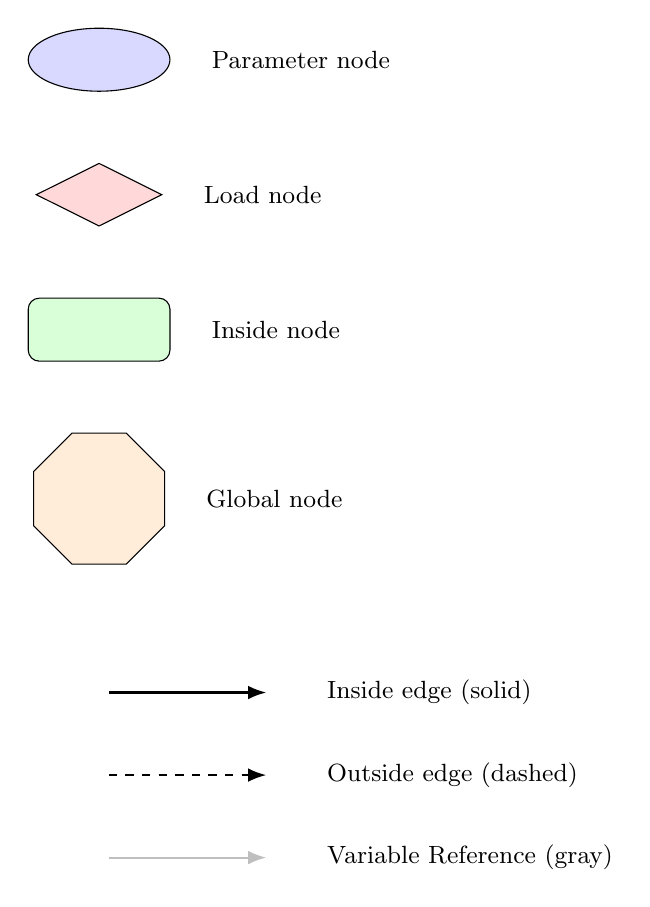
\begin{tikzpicture}[
  >=Latex,
  every node/.style={font=\small},
  param/.style={
    draw, ellipse, fill=blue!15,
    minimum width=1.8cm, minimum height=0.8cm
  },
  load/.style={
    draw, diamond, aspect=2.0, fill=red!15,
    minimum width=1.6cm, minimum height=0.8cm
  },
  inside/.style={
    draw, rectangle, rounded corners, fill=green!15,
    minimum width=1.8cm, minimum height=0.8cm
  },
  global/.style={
    draw, regular polygon, regular polygon sides=8, fill=orange!15, 
    minimum width=1.8cm, minimum height=0.8cm
  },
  insideedge/.style={->, thick},
  outsideedge/.style={->, dashed, thick},
  variablereference/.style={->, thick, gray!50}
]

% --- Node legend ---
\node[param] (p) {};
\node[right=0.4cm of p] {Parameter node};

\node[load, below=0.9cm of p] (l) {};
\node[right=0.4cm of l] {Load node};

\node[inside, below=0.9cm of l] (i) {};
\node[right=0.4cm of i] {Inside node};

\node[global, below=0.9cm of i] (g) {};
\node[right=0.4cm of g] {Global node};

% --- Edge legend ---
\node[below=1.5cm of g] (start1) {};
\node[right=2cm of start1] (end1) {};
\draw[insideedge] (start1) -- (end1);
\node[right=0.4cm of end1] {Inside edge (solid)};

\node[below=0.8cm of start1] (start2) {};
\node[right=2cm of start2] (end2) {};
\draw[outsideedge] (start2) -- (end2);
\node[right=0.4cm of end2] {Outside edge (dashed)};

\node[below=0.8cm of start2] (start3) {};
\node[right=2cm of start3] (end3) {};
\draw[variablereference] (start3) -- (end3);
\node[right=0.4cm of end3] {Variable Reference (gray)};

\end{tikzpicture}
\caption{Legend for node and edge types used in points-to graphs.}
\label{ptg-legend}
\end{figure}

\subsubsection{LUB}

When control-flow paths merge, the analysis conservatively joins the incoming states by computing the union of their nodes, edges, and write sets. This is the \emph{least upper bound} of our analysis. It ensures that the resulting abstract state over-approximates all possible executions. The join algorithm is shown in \Cref{fig:lub-code}.

An example illustrating the join operation is shown in \Cref{fig:lub-graphs}. Consider the program in \Cref{lst:lub-example}. The control-flow graph splits into two branches. On one branch, $y$ is assigned the parameter $x$, resulting in the points-to graph shown in \Cref{fig:lub-branch1}. On the other branch, $y$ is assigned a newly allocated object, producing the points-to graph shown in \Cref{fig:lub-branch2}. The two branches merge at line~7. At this point, we apply the join operation from \Cref{lst:lub-join} to obtain the combined points-to graph shown in \Cref{alias}.



\begin{figure}[ht]
\centering

% -------------------------
% Java code
% -------------------------
\begin{subfigure}{0.48\textwidth}
\begin{lstlisting}[language=Java]
static Object Lub_example(boolean p, Object x) {
    Object y;
    if (p) {
        y = x;      
    } else {
        y = new Object();
    }
    return y;
}
\end{lstlisting}
\caption{Example program used to illustrate the join.}
\label{lst:lub-example}
\end{subfigure}
\hfill
% -------------------------
% Join algorithm
% -------------------------
\begin{subfigure}{0.48\textwidth}
\begin{lstlisting}[
    basicstyle=\ttfamily\small,
    breaklines=true,
    frame=single,
    numbers=none,
    keepspaces=true,
    showstringspaces=false,
    mathescape=true
]
Join(G1, G2):
    I <- I_1 U I_2
    O <- O_1 U O_2
    L <- for each variable v:
         L(v) <- L_1(v) U L_2(v)
    E <- E_1 U E_2
    W <- W_1 U W_2
\end{lstlisting}
\caption{Definition of the LUB (join) operation.}
\label{lst:lub-join}
\end{subfigure}

\caption{Code fragments used in the join example.}
\label{fig:lub-code}
\end{figure}

\begin{figure}[ht]
\centering

% -------------------------
% Branch 1
% -------------------------
\begin{subfigure}{0.32\textwidth}
\centering
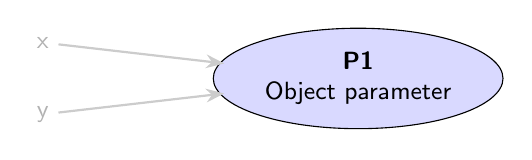
\begin{tikzpicture}[
    >=Stealth, 
    node distance=1.5cm,
    param/.style={draw, ellipse, fill=blue!15,
        minimum width=1.8cm, minimum height=0.8cm,
        align=center,
        font=\small\sffamily\bfseries},
    varlbl/.style={font=\small\sffamily, text=gray!60},
    insedge/.style={->, thick, color=gray!40, shorten >=2pt}
]
\node[param] (P1) {P1 \\ \mdseries Object parameter};
\node[varlbl, left=2.5cm of P1.north west] (I1) {x};
\node[varlbl, left=2.5cm of P1.south west] (I2) {y};
\draw[insedge] (I1) -- ($(P1.west)!0.4!(P1.north west)$);
\draw[insedge] (I2) -- ($(P1.west)!0.4!(P1.south west)$);
\end{tikzpicture}
\caption{$y = x$ branch} \label{fig:lub-branch1}
\end{subfigure}
\hfill
% -------------------------
% Branch 2
% -------------------------
\begin{subfigure}{0.32\textwidth}
\centering
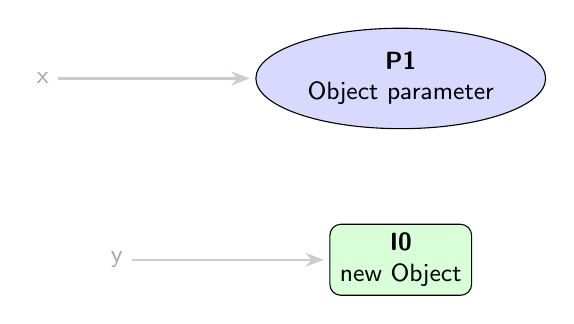
\begin{tikzpicture}[
    >=Stealth, 
    node distance=1.2cm and 2.5cm,
    allocation/.style={draw, rectangle, rounded corners, fill=green!15,
        minimum width=1.8cm, minimum height=0.8cm,
        align=center,
        font=\small\sffamily\bfseries},
    param/.style={draw, ellipse, fill=blue!15,
        minimum width=1.8cm, minimum height=0.8cm,
        align=center,
        font=\small\sffamily\bfseries},
    varlbl/.style={font=\small\sffamily, text=gray!70},
    insedge/.style={->, thick, color=gray!40, shorten >=2pt}
]
\node[param] (P1) {P1 \\ \mdseries Object parameter};
\node[allocation, below=of P1] (I0) {I0 \\ \mdseries new Object};
\node[varlbl, left=of I0] (L2) {y};
\node[varlbl, left=of P1] (L1) {x};
\draw[insedge] (L2) -- (I0);
\draw[insedge] (L1) -- (P1);
\end{tikzpicture}
\caption{$y = \texttt{new Object()}$ branch} \label{fig:lub-branch2}
\end{subfigure}
\hfill
% -------------------------
% Join result
% -------------------------
\begin{subfigure}{0.32\textwidth}
\centering
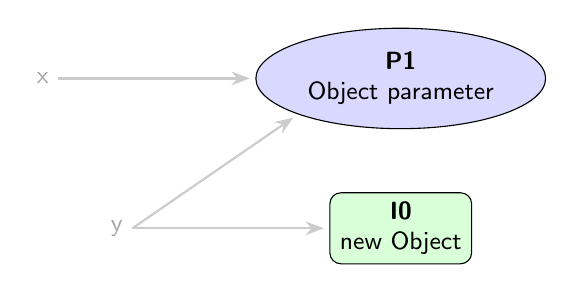
\begin{tikzpicture}[
    >=Stealth, 
    node distance=0.8cm and 2.5cm,
    allocation/.style={draw, rectangle, rounded corners, fill=green!15,
        minimum width=1.8cm, minimum height=0.8cm,
        align=center,
        font=\small\sffamily\bfseries},
    param/.style={draw, ellipse, fill=blue!15,
        minimum width=1.8cm, minimum height=0.8cm,
        align=center,
        font=\small\sffamily\bfseries},
    varlbl/.style={font=\small\sffamily, text=gray!70},
    insedge/.style={->, thick, color=gray!40, shorten >=2pt}
]

\node[param] (P1) {P1 \\ \mdseries Object parameter};
\node[allocation, below=of P1] (I0) {I0 \\ \mdseries new Object};

\node[varlbl, left=of P1] (L1) {x};
\node[varlbl, left=of I0] (L2) {y};

\draw[insedge] (L1) -- (P1);
\draw[insedge] (L2) -- (I0);
\draw[insedge] (L2.east) -- (P1.south west);

\end{tikzpicture}
\caption{Result after join} \label{alias}
\end{subfigure}

\caption{Per-branch alias graphs and their least upper bound.}
\label{fig:lub-graphs}
\end{figure}


\subsection{Analysis of Method Calls}\label{sec:method-call}

When analyzing a caller and encountering a call site of the form
\[
v_R = v_0.m(v_1,\dots,v_k),
\] there are three cases. 

\begin{enumerate}
    \item If the callee is whitelisted (known side-effect-free library method), then we can simply ignore its effect on the function.
    \item If the callee's summary is available in cache, the previously computed summary of the callee must be integrated into the caller’s current abstract state. This integration proceeds in three conceptual stages described further in Algorithm \ref{alg:graph-combination}.
    \item Conservatively, we fall back on the callee being side-effecting.
\end{enumerate}

The three steps are described in Algorithm \ref{alg:handle-interprocedural-calls}

 
\label{agl4i}
\begin{lstlisting}[
caption={Handling interprocedural calls}, 
    label={alg:handle-interprocedural-calls},
    basicstyle=\ttfamily\small,
    breaklines=true,
    frame=single,
    numbers=none,
    keepspaces=true,
    showstringspaces=false,
    mathescape=true
]
Apply(v = w.foo(a1, ..., ak), G):

    sig $\leftarrow$ method signature of foo

    if IsSafeMethod(sig) then
        // Known manually-labelled side-effect-free library method
        if v has reference type then
            n $\leftarrow$ fresh InsideNode // TODO: Ongoing optimization will handle this soundly
            strongUpdate(v, { n })
        return
   
    if cache.contains(sig) then
        // Use cached interprocedural summary
        calleeSummary $\leftarrow$ cache.get(sig)
        InstantiateSummary(G, calleeSummary, [w, a1, ..., ak], v)  // Algorithm 5
        return

    // Conservative fallback: assume the worst
    for each reference-type argument a in [w, a1, ..., ak] do
        for each node n in L(a) do
            markGlobalEscaped(n)
    if v has reference type then
        strongUpdate(v, { GlobalNode })
\end{lstlisting}


 

 
When the graph summary of the callee is available, we utilize Algorithm \ref{alg:handle-interprocedural-calls} to merge the graph of the caller at the call-point with the graph of the callee. This is done in four steps. 

\paragraph{1) Computing the Node Mapping $\mu$}

First, the analysis determines, for each abstract node in the callee's graph, which abstract nodes it corresponds to in the caller's graph.
This correspondence is captured by a node-mapping relation (from nodes to a node set). 
Intuitively, for each node in the callee summary, the mapping identifies which nodes in the caller it may represent at this particular call site.

The mapping $\mu$ is computed conservatively. 
Formal parameter nodes are mapped to the abstract objects that the caller passes as arguments. 
If the callee reads a field that the caller previously wrote, that information is propagated.
Additionally, if two callee nodes may refer to the same concrete object after argument substitution (i.e., they may alias), then effects such as stores and subsequent loads are connected accordingly. This aliasing reasoning is essential for correctly modeling interactions between different parameters when the caller passes the same object multiple times.

\paragraph{2) Projecting the Callee Summary into Caller Space}

Once the mapping is known, the callee summary is rewritten in terms of caller nodes. 
Conceptually, this step substitutes actual argument objects for the callee’s parameter placeholders. During this projection:
\begin{itemize}
    \item Inside nodes and load nodes are preserved.
    \item Parameter nodes are eliminated, because they are only placeholders for actual arguments and should not remain in the caller’s graph.
\end{itemize}

\noindent At this point, the callee’s heap effects are expressed entirely using nodes that exist in the caller’s abstract state.

\paragraph{3) Constructing the Post-Call State}

Finally, the caller’s abstract state is updated to reflect the effects of the call.

\begin{itemize}
    \item Heap writes performed by the callee are merged into the caller’s heap graph.
    \item Outside edges are merged, with their base objects rewritten into caller terms.
    \item The caller’s receiving variable (we assume 3-address code) is updated to point to the abstract nodes corresponding to the callee’s return value. 
    This step modifies variable-reference edges, not heap field edges.
    \item Escape information produced by the callee is incorporated into the caller.
\end{itemize}

\noindent After this integration, the caller’s analysis continues using the updated abstract state. 
Callee parameter nodes no longer appear in the graph; only caller nodes, inside nodes, load nodes, and global nodes remain. In this way, inter-procedural composition instantiates a context-independent method summary into a specific calling context, while preserving sound over-approximation of possible heap effects.

\paragraph{4) Simplification} Finally, a simplification step removes captured load nodes and redundant edges, preserving only those load nodes that remain reachable from escaped objects.
A summary of the algorithm is shown in Algorithm \ref{alg:graph-combination} below.

\begin{lstlisting}[
    caption={Viewpoint Adaptation}, 
    label={alg:graph-combination},
    basicstyle=\ttfamily\small,
    breaklines=true,
    frame=single,
    numbers=none,
    keepspaces=true,
    showstringspaces=false,
    mathescape=true
]
Algorithm: InstantiateSummary(G_caller, summary_callee, actualArgs, returnVar)

Input:  Caller's current graph G_caller,
        callee's exit-graph summary G_callee = (I_c, O_c, L_c, E_c, W_c),
        actual arguments [a0, ..., ak],
        variable to receive return value (may be null)
Output: G_caller updated in place

// --- Step 0: Remap callee node IDs to fresh caller-namespace IDs ---
//     (InsideNodes and LoadNodes get fresh IDs; ParameterNodes are not remapped;
//      GlobalNode maps to itself)

for each InsideNode n in G_callee do
    remap(n) $\leftarrow$ fresh InsideNode in G_caller
for each LoadNode n in G_callee do
    remap(n) $\leftarrow$ fresh LoadNode in G_caller
Apply remap to all edges, return targets, E_c, and W_c in G_callee

// --- Step 1: Compute node mapping mu (least fixed point) ---

Initialize mu:
    for i = 0, ..., k do
        mu(P_i) $\leftarrow$ pt_caller(actualArgs[i])      // Constraint 1
    for all other callee nodes n do
        mu(n) $\leftarrow$ {}

repeat until mu reach a fixed-point:
    // Constraint 2: callee outside edge meets caller inside edge
    for each outside edge (n1 --f--> n2) in O_c do
        for each node n3 in mu(n1) do
            for each node n4 in InsideEdgeTargets_caller(n3, f) do
                mu(n2) $\leftarrow$ mu(n2) $\cup$ { n4 }

    // Constraint 3: callee outside edge meets callee inside edge (aliasing)
    for each outside edge (n1 --f--> n2) in O_c do
        for each inside edge (n3 --f--> n4) in I_c do
            S1 $\leftarrow$ mu(n1) $\cup$ ({n1} \ ParameterNode)
            S3 $\leftarrow$ mu(n3) $\cup$ ({n3} \ ParameterNode)
            if S1 intersects S3 and (n1 != n3 or n1 is LoadNode) then
                mu(n2) $\leftarrow$ mu(n2) $\cup$ mu(n4) $\cup$ ({n4} \ ParameterNode)

// Extended mapping: identity for non-parameter nodes
mu'(n) = mu(n) $\cup$ ({n} \ ParameterNode)

// --- Step 2 and 3: Combine graphs ---

// Inside edges
for each inside edge (n1 --f--> n2) in I_c do
    for each n1' in mu'(n1), n2' in mu'(n2) do
        addInsideEdge_caller(n1', f, n2')

// Outside edges (skip if source maps to InsideNode)
for each outside edge (n --f--> nL) in O_c do
    for each n' in mu'(n) do
        if n' is not InsideNode then
            addOutsideEdge_caller(n', f, nL)

// Return value
if returnVar != null then
    retNodes $\leftarrow$ Union of mu'(n) for each n in returnTargets(G_callee)
    strongUpdate(returnVar, retNodes)

// Escaped nodes
E_caller $\leftarrow$ E_caller $\cup$ { n' : n in E_c, n' in mu'(n) }

// Update Write Set
for each (n, f) in W_c do
    for each n' in mu'(n) do
        if n' is not InsideNode and n' exists in G_caller then
            recordMutation_caller(n', f)

// --- Step 4: Remove captured load nodes ---
//     A LoadNode is "captured" if it is unreachable from any root
//     (parameters, global escaped nodes, variable targets).
liveNodes $\leftarrow$ BFS from roots of G_caller along all edges
for each LoadNode nL in G_caller do
    if nL not in liveNodes then
        removeNode(nL)
\end{lstlisting}

\subsection{Side-Effect Verdict} \label{sec:side-effect-verdict}
Before we infer the side-effectiveness of the method, we validate the exit points-to graph based on the following rules:
1. An inside node cannot be the source of an outside edge
2. An outside node cannot lead to an inside edge.
If either of the two rules is violated, we immediately return \texttt{GRAPH VIOLATION}.

After the graph is validated, the analysis determines side-effectiveness by inspecting the exit points-to graph and the write set. The checker accumulates \emph{all} violations into a set of reasons and reports them together. The output type of the checker is therefore either \texttt{SIDE\_EFFECT\_FREE} or \texttt{SIDE\_EFFECTING(reasons)}, where \texttt{reasons} is a \texttt{Set<String>}, a set of human-readable strings each describing one distinct violation. 


Following the algorithm of Salcianu--Rinard, we define two node sets from the exit graph. Let $\mathit{PrestateNodes}$ be the set of all nodes reachable from any parameter node by traversing only outside edges. These are the nodes that represent objects which existed before the method was called: the parameter nodes themselves plus any heap objects read from them. Let $\mathit{EscapedNodes}$ be the set of all nodes that escape. We say that a node $n$ \emph{escapes} if it is reachable from the global state --- if any part of the program outside the current method can access the object $n$ represents without going through the method's parameters. Formally, $n$ escapes if it is reachable from $E \cup \{n_{GBL}\}$ via any combination of inside and outside edges in the exit graph. Both sets are computed as graph reachability closures over the exit graph.

A node in $\mathit{PrestateNodes}$ that is also in $\mathit{EscapedNodes}$ has escaped to global scope---it was part of the heap before the call and is now accessible to the whole program, which is a side effect. Similarly, a write set entry $\langle n, f \rangle \in W$ where $n \in \mathit{PrestateNodes}$ indicates that a pre-existing heap object was mutated, which is also a side effect.

Step 3 of Algorithm~\ref{alg:sideEffectChecker} checks for mutations to the global node $n_{GBL}$ directly, as a separate step before the loop over $\mathit{PrestateNodes}$. The reason is that $n_{GBL}$ is always a member of $\mathit{EscapedNodes}$ by definition (it is the root of global state). If we added $n_{GBL}$ to $\mathit{PrestateNodes}$, every method that reads any static field would have $n_{GBL} \in \mathit{PrestateNodes} \cap \mathit{EscapedNodes}$, causing the escape check to fire and classify all such methods as side-effecting. Step 3 avoids this by checking only write set entries whose source node is $n_{GBL}$: a static field \emph{write} is a side effect, but a static field \emph{read} is not.

Constructors are treated with a limited exception to the side-effect rules. Direct field writes to the receiver object (e.g., \texttt{this.f = x}) are considered side-effect-free, since they initialize an object that is newly allocated during the constructor call. However, this exception is precise: only direct writes to fields of \texttt{this} (i.e., the parameter node $P_0$) are exempted from the mutation check. The escape check still applies---if \texttt{this} escapes to global scope even inside a constructor, that is a side effect. Writes that traverse through the receiver to reach other heap objects (e.g., \texttt{this.list.add(x)}) are treated as mutations of pre-existing state and cause the constructor to be classified as side-effecting.

This distinction follows from the definition of side effects used by the analysis. At constructor entry, the receiver object is freshly allocated and did not exist in the pre-state. Direct field assignments to \texttt{this} therefore modify only newly created state and cannot affect any heap location observable before the constructor call. In contrast, writes that traverse through the receiver may reach objects supplied as arguments or reachable from global state. Such objects may have existed before the constructor invocation, and mutating them constitutes a side effect under the pre-state mutation criterion.

After the graph-based checks above produce a verdict, there is one additional source of side-effectfulness: a method may be overridden by another method that is itself side-effecting. This matters for soundness because a call site that dispatches virtually may invoke the overriding implementation at runtime, even if the base method is side-effect-free. The analysis therefore performs an override propagation step (Step 6) after the graph-based verdict is determined. This step consults a precomputed \emph{override graph}, which maps each base method to the set of methods that override it within the set of analyzed files. If the base method passed all graph-based checks (i.e., was tentatively classified as \texttt{SIDE\_EFFECT\_FREE}), Step 6 iterates over every known override and looks it up in the summary cache. A reason of the form \emph{``overridden by side-effecting $o$''} is added to the reason set for each override $o$ that has been determined to be side-effecting. If at least one such override exists, the base method is changed to \texttt{SIDE\_EFFECTING} and all overrides are reported.

\begin{lstlisting}[
    caption={Side-effect inference},
    label={alg:sideEffectChecker},
    basicstyle=\ttfamily\small,
    breaklines=true,
    frame=single,
    numbers=none,
    keepspaces=true,
    showstringspaces=false,
    mathescape=true
]
Algorithm: CheckSideEffects(m, G_exit)

Input:  Method m, exit graph G_exit = (I, O, L, E, W)
Output: SIDE_EFFECT_FREE or SIDE_EFFECTING(reasons : Set<String>)

// Step 1: Compute PrestateNodes
//   Objects that existed before the call: parameter nodes plus all
//   nodes reachable from them via outside edges only.
PrestateNodes $\leftarrow$ reachability({ n $\in$ G_exit : n is ParameterNode }, outside edges only)

// Step 2: Compute EscapedNodes
//   A node escapes if it is reachable from global state, i.e., from
//   E $\cup$ {$n_{GBL}$} via any combination of inside and outside edges.
EscapedNodes $\leftarrow$ reachability(E $\cup$ { $n_{GBL}$ }, all edges)

// Accumulate all violations into a set of reasons
reasons $\leftarrow$ {}

// Step 3: Check for writes to static fields (mutations of $n_{GBL}$)
for each $\langle n_{GBL}$, f$\rangle$ in W do
    reasons $\leftarrow$ reasons $\cup$ { "writes to static field f" }

// Step 4: Check each prestate node for escape and mutation
for each node n in PrestateNodes do
    // Escape check: prestate node must not be globally reachable
    if n in EscapedNodes then
        reasons $\leftarrow$ reasons $\cup$ { "prestate node n escapes to global scope" }

    // Mutation check: prestate node must not appear in the write set
    for each $\langle$n, f$\rangle$ in W do
        // Constructor exception
        if m is a constructor and n = P0 then
            continue
        reasons $\leftarrow$ reasons $\cup$ { "mutates prestate node n via field f" }

// Step 5: Return verdict with all accumulated reasons
if reasons $\neq$ {} then
    return SIDE_EFFECTING(reasons)
verdict $\leftarrow$ SIDE_EFFECT_FREE

// Step 6: Override propagation
if OverrideGraph contains m then
    for each override o in OverrideGraph[m] do
        if SummaryCache[o].result = SIDE_EFFECTING then
            reasons $\leftarrow$ reasons $\cup$ { "overridden by side-effecting o" }

if reasons $\neq$ {} then
    return SIDE_EFFECTING(reasons)

return verdict
\end{lstlisting}



\input{example}


% \subsection{Illustrative example}

% \begin{figure}[H]
% \centering

% % (a) Code
% \begin{subfigure}[t]{\textwidth}
% \begin{lstlisting}
% class BankAccount {
%     int balance;
%     BankAccount(int initialBalance) {
%         this.balance = initialBalance;
%     }
%     void deposit(int amount) {
%         this.balance += amount;
%     }
% }

% class Wallet {
%     BankAccount account;
%     Wallet(BankAccount account) {
%         this.account = account;
%     }
%     void addFunds(int amount) {
%         this.account.balance += amount;
%     }
% }
% \end{lstlisting}
% \caption{Example program.}
% \label{fig:purity-example-code}
% \end{subfigure}

% \vspace{1em}

% % (b) Points-to graph
% \begin{subfigure}[H]{\textwidth}
% \centering
% \begin{tikzpicture}[
%   >=Latex,
%   every node/.style={font=\small},
%   param/.style={
%     draw, ellipse, fill=blue!15,
%     minimum width=3.2cm, minimum height=1.1cm, align=center
%   },
%   load/.style={
%     draw, diamond, aspect=2.0, fill=red!15,
%     minimum width=2.8cm, minimum height=1.1cm, align=center
%   },
%   outsideedge/.style={->, dashed, thick},
%   inside/.style={
%     draw, rectangle, rounded corners, fill=green!12,
%     minimum width=3.0cm, minimum height=1.0cm, align=center
%   }
% ]

% % Nodes
% \node[param] (P0) {P$_0$\\ \texttt{this : Wallet}};
% \node[load, right=3.6cm of P0] (L0) {L$_0$\\ \texttt{BankAccount}};

% % Outside edge
% \draw[outsideedge] (P0) -- node[above]{\texttt{account}} (L0);

% % Mutation set
% \node[below=0.5cm of L0, align=center]
% {$W = \{(L_0,\ \texttt{balance})\}$};

% \end{tikzpicture}
% \caption{Points-to graph at the statement
% \texttt{this.account.balance += amount} in \texttt{Wallet.addFunds}.
% $W$ denotes the write set.}
% \label{fig:purity-example-graph}
% \end{subfigure}

% \caption{Illustrative side-effect analysis example.
% (a) A simple program modeling a bank account and a wallet.
% (b) Points-to graph for the field update in \texttt{Wallet.addFunds}.
% }
% \label{fig:purity-example}
% \end{figure}

% To illustrate the analysis, consider the code in \Cref{fig:purity-example-code}. At line 17, the \texttt{addFunds} method mutates the balance of the
% \texttt{BankAccount} object reachable from the receiver via field \texttt{account}. The corresponding points-to graph is shown in \Cref{fig:purity-example-graph}. The receiver $P_0$ is a parameter node. Accessing field \texttt{account} introduces a load node $L_0$ representing a
% pre-existing heap object. Mutating field \texttt{balance} of $L_0$ records $(L_0,\texttt{balance})$ in the write set. Because $L_0$ represents a pre-existing object, this mutation causes the method to be classified as impure.

\section{Implementation}



\begin{figure}[H]
\centering
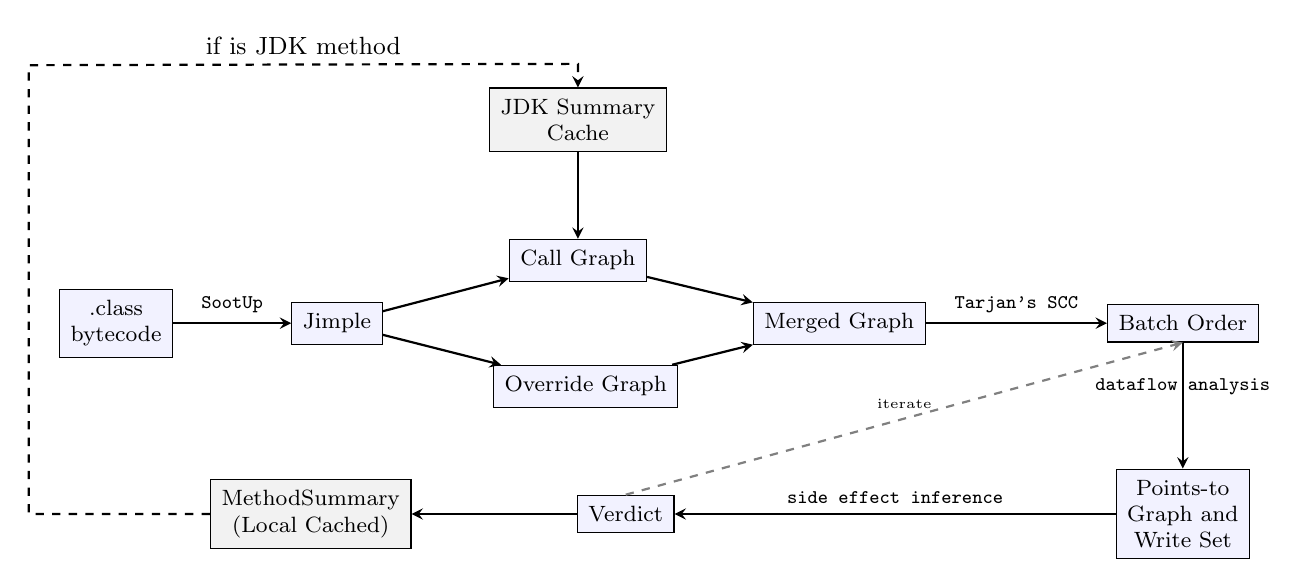
\begin{tikzpicture}[
    node distance=1.1cm, 
    artifact/.style={rectangle, draw, fill=blue!5, font=\footnotesize, inner sep=4pt, align=center},
    process/.style={rectangle, draw, fill=orange!5, font=\footnotesize\itshape, inner sep=4pt, align=center},
    verdict/.style={rectangle, draw, fill=green!10, rounded corners, font=\footnotesize\bfseries, inner sep=4pt, align=center},
    arrow/.style={thick, ->, >=stealth}
]

% --- FIRST LINE ---
\node (bytecode) [artifact] {.class\\bytecode};
\node (soot)     [artifact, right=of bytecode, xshift=0.4cm] {Jimple};
\node (callgen)  [artifact, right=of soot, xshift=0.5cm, yshift=0.8cm] {Call Graph};
\node (overridegen) [artifact, right=of soot,xshift=0.3cm, yshift=-0.8cm] {Override Graph};
\node (cg)       [artifact, right=of soot, xshift=3.6cm, ] {Merged Graph};
\node (jdk_cache) [artifact, above=of callgen, fill=gray!10] {JDK Summary\\Cache};

% --- SECOND LINE (Positioned below the CallGraph) ---
\node (loop)     [artifact, right=of cg, xshift=1.2cm] {Batch Order};
\node (ptg)      [artifact, below=of loop, yshift=-0.5cm] {Points-to\\Graph and\\Write Set};

% Final split outputs
\node (verdict)  [artifact,  left=of ptg, xshift=-4.5cm] {Verdict};
\node (summary)  [artifact, left=of verdict, xshift=-1.0cm, fill=gray!10] {MethodSummary\\(Local Cached)};

% --- PATHS ---
% Top row connections
\draw [arrow] (bytecode) -- node[above, font=\scriptsize\ttfamily] {SootUp} (soot);
\draw [arrow] (soot) -- (callgen);
\draw [arrow] (soot) -- (overridegen);
\draw [arrow] (jdk_cache.south) -- (callgen.north);
\draw [arrow] (callgen) -- (cg);
\draw [arrow] (overridegen) -- (cg);

% Connection between rows (The "Snake" turn)
\draw [arrow] (cg) -- node[above, font=\scriptsize\ttfamily, align=center] {Tarjan's SCC}(loop);

% Bottom row connections (Moving right to left)
\draw [arrow] (loop) -- node[above, font=\scriptsize\ttfamily, align=center] {dataflow analysis}  (ptg);
\draw [arrow] (ptg) -- node[above, font=\scriptsize\ttfamily, align=center] {side effect inference} (verdict);

% Caching connection
\draw [arrow] (verdict) -- (summary);
\draw [arrow, dashed] (summary.west) 
    -- ++(-2.3,0) 
    -- ++(0,5.7) 
    -- ([yshift=0.3cm]jdk_cache.north) 
    node[midway, above, font=\small] {if is JDK method} 
    -- (jdk_cache.north);

% Feedback loop back to the loop node for next method
\draw [arrow, dashed, gray] (verdict.north) -- (loop.south)
    node[pos=0.5, above, font=\tiny, black] {iterate};

\end{tikzpicture}
\caption{Flow Chart of Implementation}
\label{fig:implement-flowchart}
\end{figure}

The implementation is organized into a sequence of analysis stages, as shown in Figure \ref{fig:implement-flowchart}. After we obtain the Jimple representation of the code using Sootup, we follow Algorithm \ref{alg:side-effect-analysis} as our top-level implementation. The methods are ordered so that the callees are analyzed before the callers. Mutually recursive methods form a strongly connected component (SCC) and are analyzed together. In particular, we obtain the batch order by first computing the call graph from the method signatures, and then using Tarjan's algorithm to find all sub-complete graphs.


Our implementation will output each method in the input file with its verdict result. For example, called with \texttt{Wallet.swapAccount} method \Cref{fig:example-code}, outputs:

\begin{alltt} 
\textcolor{violet}{
=== Side-Effect Analysis Results ===
testcases.reportBankExample2\$Wallet.swapAccount(java.lang.Object)         
                    : SIDE_EFFECTING (mutates this via field account)}
\end{alltt}

\subsection{SootUp}

 The analysis operates on Java bytecode via the Jimple intermediate representation and is built on top of the SootUp framework. SootUp is a Java static analysis library that 
  provides facilities for loading Java bytecode, lifting it to the Jimple three-address IR, and constructing control flow graphs; it is a redesign of the widely used Soot framework with an immutable, thread-safe API. 
  
   Jimple representation offers several properties that make it well-suited for pointer and escape analysis. First, Jimple is a three-address, register-based IR: a stack-based bytecode sequence like \texttt{iload\_1; iload\_2; iadd; istore\_3} becomes the explicit assignment \texttt{\$i0 = a + b; x = \$i0}, eliminating the need
  to simulate the operand stack. Second, Jimple performs type splitting, guaranteeing that every local variable has exactly one type throughout its lifespan; this allows the analysis to distinguish reference types from primitives with a simple type check, which is critical for deciding when to create pointer graph nodes. Third, Jimple decomposes each bytecode instruction into a typed statement object (\texttt{JAssignStmt}, \texttt{JIdentityStmt}, \texttt{JInvokeStmt}, \texttt{JReturnStmt}), with structured sub-expressions for field accesses (\texttt{JInstanceFieldRef},
  \texttt{JStaticFieldRef}), allocations (\texttt{JNewExpr}), casts, and array references. This yields a direct one-to-one correspondence between Jimple statement types and the transfer function rules
   of the Salcianu--Rinard analysis. Finally, SootUp automatically constructs a control flow graph (\texttt{StmtGraph}) from the bytecode and provides a ForwardFlowAnalysis framework that handles fixed-point iteration, join-point merging, and worklist management, so our implementation only needs to supply the transfer function and the lattice join operator.

\subsection{JDK Summary Cache}                                                   Analyzing user code inevitably requires resolving calls into the JDK standard library. Rather than re-analyzing library methods on every invocation, we persist method summaries to a disk-backed JSON  cache (\texttt{jdk-cache/}). When a cross-file callee is encountered during call graph construction or dataflow analysis, the tool consults this cache. When the analysis build call graph, the process stop either when the method is entirely self-contained (no method calls) or calls only JDK methods that its summary is already avaliable.  We ship a pre-computed cache covering common \texttt{java.util}, \texttt{java.lang}, and \texttt{java.io} methods, so that users benefit from library-level precision out of the box without incurring the cost of whole JDK analysis.  

\subsection{Handling Method Overrides}
\label{sec:override-analysis}

When multiple classes are analyzed together, the analysis detects override relationships between methods and incorporates them into the call graph. If a subclass method has the same sub-signature as a concrete method in its superclass, it is recorded as an override. The call graph is augmented so that overriding methods are analyzed before their base method and callers are analyzed after all implementations are known. 

If an overriding implementation is classified as \texttt{SIDE\_EFFECTING}, the base method is conservatively upgraded to \texttt{SIDE\_EFFECTING} when its summary is stored. This ensures that the base method summary reflects the worst-case behavior of all possible implementations that may be invoked through dynamic dispatch.

At a virtual dispatch site (e.g., \texttt{obj.m()} where the static type of \texttt{obj} is a superclass), the analysis applies the summaries of all known implementations of the method. A call is classified as \texttt{SIDE\_EFFECT\_FREE} only if all implementations are side-effect-free; if any implementation mutates pre-existing state, the call is classified as \texttt{SIDE\_EFFECTING}. This mechanism applies only to classes included in the analysis input; calls to external libraries continue to use the existing resolution strategy. 

For an illustrative example, consider the classes in \Cref{fig:override-example-code}. In \texttt{OverrideBase}, method \texttt{process} only reads the field \texttt{this.value} and is therefore side-effect-free when analyzed in isolation. In \texttt{OverrideDerived}, the overridden method writes to \texttt{this.value}. Since \texttt{this} is a pre-existing receiver object, this mutation makes \texttt{OverrideDerived.process(Object)} \texttt{SIDE\_EFFECTING}. Because the base method is overridden by a side-effecting implementation, its verdict is conservatively upgraded to \texttt{SIDE\_EFFECTING}. Method \texttt{OverrideBase.caller(OverrideBase,Object)} performs a virtual dispatch through \texttt{b.process(input)}. Since the receiver \texttt{b} may refer to either class, the analysis applies the summaries of both implementations. Because one implementation is side-effecting, the call and the caller are both classified as \texttt{SIDE\_EFFECTING}. The resulting override and call relationships are illustrated in \Cref{fig:override-example-graph}.

\begin{figure}[H]
\centering
\begin{subfigure}[t]{0.48\textwidth}
\begin{lstlisting}[language=Java]
class OverrideBase {
    Object value;

    OverrideBase(Object v) {
        this.value = v;
    }

    Object process(Object input) {
        return this.value;
    }

    Object caller(OverrideBase b,
                  Object input) {
        return b.process(input);
    }
}
\end{lstlisting}
\caption{\texttt{OverrideBase.java}}
\end{subfigure}
\hfill
\begin{subfigure}[t]{0.48\textwidth}
\begin{lstlisting}[language=Java]
class OverrideDerived
    extends OverrideBase {

    OverrideDerived(Object v) {
        super(v);
    }

    @Override
    Object process(Object input) {
        this.value = input;
        return this.value;
    }
}
\end{lstlisting}
\caption{\texttt{OverrideDerived.java}}
\end{subfigure}
\caption{Example used to illustrate override-aware inter-file analysis.}
\label{fig:override-example-code}
\end{figure}

\begin{figure}[t]
\centering
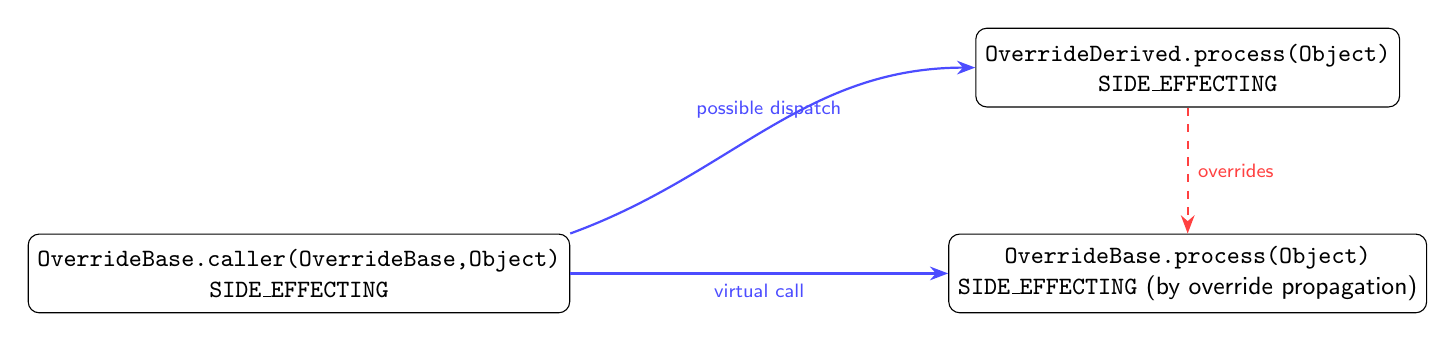
\begin{tikzpicture}[
    >=Stealth,
    node distance=1.6cm and 2.6cm,
    method/.style={
        draw,
        rounded corners,
        align=center,
        minimum width=4.0cm,
        minimum height=1.0cm,
        font=\small\sffamily
    },
    call/.style={->, thick, blue!70},
    override/.style={->, thick, red!75, dashed}
]

\node[method] (derived) {\texttt{OverrideDerived.process(Object)}\\\texttt{SIDE\_EFFECTING}};
\node[method, below=of derived] (base) {\texttt{OverrideBase.process(Object)}\\\texttt{SIDE\_EFFECTING} (by override propagation)};
\node[method, left=4.8cm of base] (caller) {\texttt{OverrideBase.caller(OverrideBase,Object)}\\\texttt{SIDE\_EFFECTING}};

\draw[override] (derived) -- node[right, font=\scriptsize\sffamily] {overrides} (base);
\draw[call] (caller) -- node[below, font=\scriptsize\sffamily] {virtual call} (base);
\draw[call] (caller.north east) to[out=20,in=180] node[above, font=\scriptsize\sffamily] {possible dispatch} (derived.west);

\end{tikzpicture}
\caption{Override-aware dependency graph for the example. Blue edges denote call relationships; the red dashed edge denotes an override relationship. Because the virtual call in \texttt{caller} may dispatch to either implementation, and \texttt{OverrideDerived.process(Object)} is side-effecting, both \texttt{OverrideBase.process(Object)} and \texttt{OverrideBase.caller(OverrideBase,Object)} are classified as \texttt{SIDE\_EFFECTING}.}
\label{fig:override-example-graph}
\end{figure}


\input{evaluation}





% Scalability:

% Runtime per package and total runtime.

% Peak memory per package and total.

% Basic size metrics for context (e.g., number of analyzed methods, call-graph edges) to normalize comparisons.

% Direct consumability:

% Stub generation success: percent of methods for which we can emit well-formed purity annotations/stubs.

% Integration success: whether the generated stubs compile and can be consumed by the Checker Framework without manual edits (pass/fail plus any failure categories).

% Downstream impact:

% Run one or more Checker Framework clients (at minimum the purity/effects checking itself, and ideally a flow-sensitive client like Nullness or a modifiability-style checker) on selected Java projects under two conditions: (A) current JDK purity specs, and (B) current specs plus our inferred purity stubs.

% Compare: total warnings and distinct warning sites; reduction in warnings attributable to lost flow refinements across calls; and any regressions (new warnings or type-check failures).
% Falsifiability: if the analysis does not scale to core packages, if generated stubs require substantial manual editing to use, or if downstream warning reduction is negligible, RQ3 is not supported.

% Planned result presentation.

% A table per package: total methods analyzed; counts of Pure/SideEffectFree/Deterministic; and baseline vs fresh-aware deltas.

% A chart of runtime and peak memory per package (baseline vs fresh-aware).

% A table of audited precision with confidence intervals and a taxonomy of false positives/false negatives.

% A before/after table (and optionally a bar chart) of Checker Framework warning counts on downstream projects, highlighting reductions due to preserved flow-sensitive facts.




\bibliographystyle{plain}
\bibliography{refs}

% As always, use a descriptive title (not "project proposal"). If a UI is an important part of your project, draw a mockup of it. Avoid vague, content-free verbs liko "to leverage" or "to utilize". Be specific.

\newpage
\appendix


\end{document}
